\documentclass[a4paper]{amsart}

\usepackage[margin=1in]{geometry}
\usepackage{amsmath,amssymb,mathtools}
\usepackage{tikz}
\usepackage{microtype}
\usepackage[hidelinks]{hyperref}

\newtheorem{theorem}{Theorem}[section]
\newtheorem{lemma}[theorem]{Lemma}
\theoremstyle{remark}
\newtheorem{remark}[theorem]{Remark}

\newcommand{\qd}{d_{\mathrm Q}}
\newcommand{\pat}{\operatorname{pat}}
\newcommand{\E}{\mathbb E}
\newcommand{\Prb}{\mathbb P}
\newcommand{\Dih}{\mathcal D}

\title{Maximum Quartet Distance}
\date{}
\subjclass[2020]{05C35, 05A05, 92D15}
\keywords{quartet distance, phylogenetic tree, permuton,
permutation pattern, rotation system}

\begin{document}

\begin{abstract}
Let $M_n$ be the maximum quartet distance between two unrooted binary
phylogenetic trees on a common $n$-element leaf set. We prove, for every
$n\ge4$,
\[
 \frac23\binom n4
 \le M_n
 \le \min\left\{\binom n4,
 \frac23\binom n4+\frac{n(6n^2-11n+6)}9\right\}.
\]
Consequently,
$M_n=(2/3+O(n^{-1}))\binom n4$, proving the Bandelt--Dress
conjecture. The proof combines a sharp inequality for eight dihedral
four-point permutation patterns with random rotation systems of
phylogenetic trees. Under the latter randomization, the quartet displayed
by a tree is never the crossing split, while each of the other two splits
is the crossing split with probability $1/2$.
\end{abstract}

\maketitle

\section{Introduction}

An unrooted binary phylogenetic tree on a finite set $X$ is a finite
tree whose degree-one vertices are bijectively labelled by $X$ and
whose remaining vertices have degree three. For $Q\in\binom X4$,
suppressing the degree-two vertices in the minimal subtree spanning
$Q$ gives one of the three quartet topologies on $Q$; denote it by
$q_T(Q)$. The quartet distance between two such trees is
\[
 \qd(T_1,T_2)
 =
 \bigl|\{Q\in\tbinom X4:q_{T_1}(Q)\ne q_{T_2}(Q)\}\bigr|.
\]
Writing $M_n$ for the maximum of this quantity over pairs of trees on
a common $n$-element leaf set, Bandelt and Dress conjectured that
\[
 M_n=\left(\frac23+o(1)\right)\binom n4
 \qquad\text{as }n\to\infty
\]
\cite{BandeltDress}.

The conjecture has a substantial history. Alon, Snir, and Yuster
proved the general upper bound
$(9/10+o(1))\binom n4$ and obtained finite improvements over the
standard random-labelling lower bound \cite{AlonSnirYuster}.
Alon, Naves, and Sudakov subsequently improved the general upper bound
to $(0.69+o(1))\binom n4$ and proved the conjecture for pairs of
caterpillar trees \cite{AlonNavesSudakov}. Chor, Erd\H{o}s, and
Komornik gave a strongly explicit construction with distance
$(2/3+o(1))\binom n4$, always exceeding the basic $2/3$ benchmark in
their family \cite{ChorErdosKomornik}. Snir, Weissberg, and Yuster
studied the related problem when part of the leaf labelling is fixed
\cite{SnirWeissbergYuster}. The general conjecture was still recorded
as open in recent work on metrics for phylogenetic tree space
\cite{CzabarkaEtAl}.

Permutation patterns already enter the caterpillar case. The proof of
Alon, Naves, and Sudakov reduces that case to a $1/3$ lower bound for
the total density of the eight patterns
\[
 \{1234,1243,2134,2143,3412,4312,3421,4321\}.
\]
The eight patterns used in the present paper are different: they form
the dihedral orbit of $1234$. The new step is a randomized
circular-order representation that applies to every binary
phylogenetic tree, not only to caterpillars. Equal crossing splits of
two circular orders are exactly detected by the dihedral pattern set,
and random rotation systems connect those crossing splits to the
quartets displayed by the original trees.

\begin{theorem}\label{thm:main}
For every integer $n\ge4$,
\[
 \frac23\binom n4
 \le M_n
 \le \min\left\{\binom n4,
 \frac23\binom n4+\frac{n(6n^2-11n+6)}9\right\}.
\]
Equivalently, the nontrivial upper estimate may be written as
\[
 \frac{M_n}{\binom n4}
 \le
 \frac23+
 \frac{8(6n^2-11n+6)}{3(n-1)(n-2)(n-3)}
 =
 \frac23+\frac{16}{n}+\frac{200}{3n^2}+O(n^{-3}).
\]
In particular,
\[
 M_n=\left(\frac23+O\left(\frac1n\right)\right)\binom n4.
\]
\end{theorem}

Here is the proof in outline. A circular order on four leaves selects
the split joining opposite positions, which we call its crossing
split. A theorem of Chan, Kr\'al', Noel, Pehova, Sharifzadeh, and
Volec implies that any two circular orders on $n$ elements have the
same crossing split on at least
$(1/3-O(1/n))\binom n4$ four-subsets. On the other hand, choose a
uniform random cyclic order of the three incident edges at every
internal vertex of a phylogenetic tree. For any fixed quartet, the
split displayed by the tree is then the unique split that can never be
the crossing split; the other two splits occur with probability
$1/2$ each. Thus, if two trees disagree on a proportion $d$ of their
quartets, their random circular orders have the same crossing split on
an expected proportion
\[
 \frac12(1-d)+\frac14d=\frac12-\frac d4.
\]
Comparison with the circular-order lower bound gives
$d\le2/3+O(1/n)$.

The sole non-elementary input is the published permuton inequality
from \cite[Theorem~7]{ChanEtAl}. We give the complete reduction from
that inequality to Theorem~\ref{thm:main}, including the finite-size
error. The argument never assumes independence among the quartet
variables associated with different four-subsets; it uses only the
one-quartet distribution and linearity of expectation.

\section{Circular orders and permutation patterns}

By a circular order on $X$ we mean an equivalence class of linear
arrangements under cyclic shifts and reversal. If the restriction of
a circular order $C$ to $Q=\{a,b,c,d\}$ has representative
$(a,b,c,d)$, define its crossing split by $\chi_C(Q)=ac\mid bd$.
This is well defined because cyclic shifts and reversal preserve the
pair of opposite positions. For two circular orders $C,C'$ on $X$,
put
\[
 K(C,C')
 =
 \bigl|\{Q\in\tbinom X4:\chi_C(Q)=\chi_{C'}(Q)\}\bigr|.
\]
Let
\[
 \Dih
 =
 \{1234,1432,2143,2341,3214,3412,4123,4321\}
 \subset S_4.
\]
Thus $\Dih$ consists of the four cyclic shifts of $1234$ and their
reversals. Equivalently, it is the dihedral subgroup of $S_4$
generated by $2341$ and $4321$; in particular, $\Dih$ is
inverse-closed.

\begin{lemma}\label{lem:relative-permutation}
Let $C,C'$ be circular orders on an $n$-element set. Choose
representatives $C=(x_1,\ldots,x_n)$ and $C'$, and let $\pi(i)$ be
the position of $x_i$ in the chosen representative of $C'$. If
$i_1<i_2<i_3<i_4$ and
$Q=\{x_{i_1},x_{i_2},x_{i_3},x_{i_4}\}$, then
\[
 \chi_C(Q)=\chi_{C'}(Q)
 \quad\Longleftrightarrow\quad
 \pat\bigl(\pi(i_1),\pi(i_2),\pi(i_3),\pi(i_4)\bigr)\in\Dih.
\]
\end{lemma}

\begin{proof}
On four labelled elements there are exactly three circular orders and
exactly three splits into two unordered pairs. Sending a circular
order to the split formed by opposite positions is a bijection.
Consequently, two restricted circular orders have the same crossing
split precisely when they differ by a cyclic shift or reversal.

Set
\[
 \sigma
 =
 \pat\bigl(\pi(i_1),\pi(i_2),\pi(i_3),\pi(i_4)\bigr).
\]
The order in which the four elements occur in $C'$ is described by
$\sigma^{-1}$. Hence the two restricted circular orders agree up to a
cyclic shift or reversal precisely when $\sigma^{-1}\in\Dih$. Since
$\Dih$ is inverse-closed, this is equivalent to $\sigma\in\Dih$.
\end{proof}

A permuton is a Borel probability measure $\mu$ on $[0,1]^2$ with
uniform marginals. For $\sigma\in S_k$, its density
$d(\sigma,\mu)$ is the probability that, after $k$ independent
points sampled from $\mu$ are ordered by increasing first coordinate,
the relative order of their second coordinates is $\sigma$. Uniform
marginals imply that ties occur with probability zero.

\begin{theorem}[Chan--Kr\'al'--Noel--Pehova--Sharifzadeh--Volec]
\label{thm:permuton}
For every permuton $\mu$,
\[
 \sum_{\sigma\in\Dih}d(\sigma,\mu)\ge\frac13.
\]
\end{theorem}

This is \cite[Theorem~7]{ChanEtAl}; its equality characterization is
not needed here.

Write
\[
 (n)_4=n(n-1)(n-2)(n-3),
 \qquad
 \alpha_n=\frac{(n)_4}{n^4}
 =\frac{(n-1)(n-2)(n-3)}{n^3}.
\]

\begin{lemma}\label{lem:circular-bound}
For any two circular orders $C,C'$ on an $n$-element set, where
$n\ge4$,
\[
 K(C,C')
 \ge
 \left(1-\frac{2}{3\alpha_n}\right)\binom n4.
\]
\end{lemma}

\begin{proof}
Let $\pi\in S_n$ be the relative permutation from
Lemma~\ref{lem:relative-permutation}, and set
\[
 I_i=\left[\frac{i-1}{n},\frac{i}{n}\right)
 \quad (1\le i\le n),
\]
with the harmless convention that $1\in I_n$. Define the step
permuton $\mu_\pi$ to have density $n$ on
\[
 \bigcup_{i=1}^n I_i\times I_{\pi(i)}
\]
and density zero elsewhere. For almost every first coordinate, the
density integrates to one along the corresponding vertical section.
The analogous statement holds horizontally, so both marginals are
uniform.

Sample four independent points from $\mu_\pi$, let $\Sigma$ be
their induced four-point pattern, and let $E$ be the event that their
first coordinates lie in four distinct intervals $I_i$. The four
strip indices are independent and uniform on $[n]$, and therefore
$\Prb(E)=\alpha_n$. Conditional on $E$, their increasing sequence is
the increasing enumeration of a uniformly random four-subset of
$[n]$. Since $\pi$ is injective, distinct first-coordinate strips
correspond to distinct second-coordinate strips; consequently, the
within-strip coordinates cannot change the induced pattern. Thus
$\Sigma$ is the four-point pattern of $\pi$ on that uniformly random
four-subset. Lemma~\ref{lem:relative-permutation} gives
\[
 p:=\Prb(\Sigma\in\Dih\mid E)
   =\frac{K(C,C')}{\binom n4}.
\]
If $r:=\Prb(\Sigma\in\Dih\mid E^c)$, then $0\le r\le1$.
Theorem~\ref{thm:permuton} consequently implies
\[
 \frac13
 \le \alpha_np+(1-\alpha_n)r
 \le \alpha_np+1-\alpha_n,
 \qquad
 p\ge1-\frac{2}{3\alpha_n}.
\]
Multiplying by $\binom n4$ proves the assertion.
\end{proof}

\section{Random rotation systems}

At every internal vertex of an unrooted binary phylogenetic tree
$T$, choose one of the two cyclic orders of its three incident edges.
Such a collection $\rho$ is a rotation system, or equivalently an
oriented ribbon structure, on $T$. A regular neighbourhood of the
resulting ribbon tree is an oriented surface that deformation
retracts onto $T$. Since $T$ is a tree, this neighbourhood is a disk.
The leaf caps therefore occur along its boundary in a cyclic order;
after forgetting the orientation, write this circular order as
$C_\rho$. Choosing the two cyclic orders independently and uniformly
at all internal vertices gives the random circular order $C_T$.

\begin{lemma}\label{lem:edge-interval}
For every deterministic rotation system $\rho$ on $T$ and every edge
$e$, the leaves in each component of $T-e$ form a circular interval
in $C_\rho$.
\end{lemma}

\begin{proof}
Cut the regular neighbourhood of $T$ across the rectangular band
corresponding to $e$. The thickening of either component of $T-e$
meets the original boundary in one arc whose endpoints lie on the two
sides of that band. All leaf caps belonging to that component occur
on this arc, and no other leaf cap does. They are therefore
consecutive in the induced circular order.
\end{proof}

For $Y\subseteq X$, let $T[Y]$ be the minimal connected subtree of
$T$ spanning $Y$, and let $T|Y$ be obtained from $T[Y]$ by
suppressing every degree-two vertex. The ribbon structure on $T$
induces one on $T|Y$: delete the unused incident bands, and replace
each maximal chain of degree-two vertices by a single band. Notice
that a cyclic order on two half-edges is unique, so no additional
choice or reversal is introduced by this suppression.

\begin{lemma}[Restriction of the boundary order]
\label{lem:restriction}
For every rotation system $\rho$ on $T$ and every subset $Y$ of its
leaves with $|Y|\ge2$, the boundary order of the induced ribbon tree
$T|Y$ is the restriction $C_\rho|Y$.
\end{lemma}

\begin{proof}
Delete the components of $T-T[Y]$ one at a time. Each deleted
component attaches to the surviving subtree through a single edge.
By Lemma~\ref{lem:edge-interval}, its leaf caps occupy one boundary
interval. Removing its thickening and closing the exposed boundary
therefore deletes exactly that interval from the cyclic list of leaf
caps and does not change the relative cyclic order of the surviving
caps. After all such components have been removed, the boundary order
is $C_\rho|Y$.

It remains to suppress degree-two vertices. Locally, the thickening
of a degree-two vertex consists of a vertex disk joined to two bands.
Replacing this disk and the two bands by one band is an
orientation-preserving isotopy away from the leaf caps. It therefore
does not change their cyclic order. Repeating this operation gives
the asserted boundary order on $T|Y$.
\end{proof}

\begin{lemma}\label{lem:wrong-channel}
Fix $Q\in\binom X4$ and a quartet topology $s$ on $Q$. For the
random circular order $C_T$,
\[
 \Prb\bigl(\chi_{C_T}(Q)=s\bigr)
 =
 \begin{cases}
  0, & s=q_T(Q),\\[2pt]
  \frac12, & s\ne q_T(Q).
 \end{cases}
\]
\end{lemma}

\begin{proof}
Write $q_T(Q)=ab\mid cd$. An edge on the path between the two branch
vertices of the induced quartet separates $\{a,b\}$ from
$\{c,d\}$. By Lemma~\ref{lem:edge-interval}, each pair is a circular
interval in $C_T|Q$. Hence $ab\mid cd$ cannot be the crossing split.

By Lemma~\ref{lem:restriction}, the restricted circular order is the
boundary order of the induced ribbon quartet $T|Q$. This quartet has
two branch vertices $u,v$, where $u$ is incident with the paths to
$a,b,v$ and $v$ is incident with the paths to $c,d,u$. Using cyclic
notation, the choices at $u$ are $(a,b,v)$ and $(a,v,b)$, while those
at $v$ are $(c,d,u)$ and $(c,u,d)$. The four pairs of choices are
equally likely: $u$ and $v$ are distinct internal vertices of the
original tree, so their induced cyclic orders remain independent
uniform choices. Rotations at vertices suppressed to degree two have
no effect, since a cyclic order on two half-edges is unique. A boundary
traversal gives the four outcomes shown in
Figure~\ref{fig:quartet-rotations}.

\begin{figure}[t]
\centering
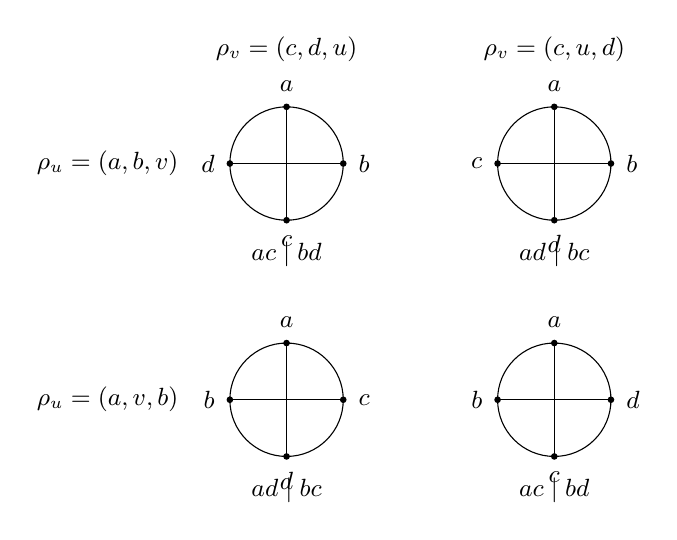
\begin{tikzpicture}[every node/.style={font=\small}]
\newcommand{\orderdiagram}[7]{%
  \begin{scope}[shift={(#1,#2)}]
    \draw (0,0) circle (0.72);
    \fill (0,0.72) circle (1.2pt) node[above=2pt] {$#3$};
    \fill (0.72,0) circle (1.2pt) node[right=2pt] {$#4$};
    \fill (0,-0.72) circle (1.2pt) node[below=2pt] {$#5$};
    \fill (-0.72,0) circle (1.2pt) node[left=2pt] {$#6$};
    \draw (0,0.72)--(0,-0.72);
    \draw (-0.72,0)--(0.72,0);
    \node at (0,-1.15) {$#7$};
  \end{scope}}

\node at (0,1.45) {$\rho_v=(c,d,u)$};
\node at (3.4,1.45) {$\rho_v=(c,u,d)$};
\node[anchor=east,align=right] at (-1.25,0)
  {$\rho_u=(a,b,v)$};
\node[anchor=east,align=right] at (-1.25,-3)
  {$\rho_u=(a,v,b)$};

\orderdiagram{0}{0}{a}{b}{c}{d}{ac\mid bd}
\orderdiagram{3.4}{0}{a}{b}{d}{c}{ad\mid bc}
\orderdiagram{0}{-3}{a}{c}{d}{b}{ad\mid bc}
\orderdiagram{3.4}{-3}{a}{d}{c}{b}{ac\mid bd}
\end{tikzpicture}
\caption{The four rotation choices for an induced quartet with true
split $ab\mid cd$. In each circle the labels are shown in boundary
order, and the two diameters join opposite positions; the split below
the circle is therefore the crossing split.}
\label{fig:quartet-rotations}
\end{figure}

Thus the two topologies distinct from $ab\mid cd$ each occur as the
crossing split in exactly two of the four cases, and hence with
probability $1/2$.
\end{proof}

\section{Proof of the theorem}

\begin{proof}[Proof of Theorem~\ref{thm:main}]
Let $T_1,T_2$ be binary phylogenetic trees on the same $n$-element
leaf set, and put $N=\binom n4$. Let $A$ be the number of
four-subsets on which the trees agree and let
\[
 D=\qd(T_1,T_2)=N-A.
\]
Choose the rotation systems of $T_1$ and $T_2$ independently,
obtaining circular orders $C_1,C_2$.

Suppose first that $q_{T_1}(Q)=q_{T_2}(Q)$. By
Lemma~\ref{lem:wrong-channel}, the random variables
$\chi_{C_1}(Q)$ and $\chi_{C_2}(Q)$ are independent uniform choices
from the same two-element set, and hence agree with probability
$1/2$. If the two true quartet topologies differ, their two supports
have exactly one topology in common, so the crossing splits agree
with probability $1/4$. Linearity of expectation gives
\[
 \E K(C_1,C_2)
 =\frac12A+\frac14D
 =\frac{N+A}{4}.
\]
No independence between the contributions of distinct four-subsets
is used here.

Lemma~\ref{lem:circular-bound} holds for every realization of
$(C_1,C_2)$ and therefore also after taking expectations. Using
$\alpha_n=(n-1)(n-2)(n-3)/n^3$, we obtain
\[
 \frac{N+A}{4}
 \ge
 \left(1-\frac{2}{3\alpha_n}\right)N,
 \qquad
 D=N-A
 \le
 \left(\frac{8}{3\alpha_n}-2\right)N.
\]
Since
\[
 1-\alpha_n=\frac{6n^2-11n+6}{n^3},
 \qquad
 \frac{N}{\alpha_n}=\frac{n^4}{24},
\]
the last bound becomes
\[
 D
 \le
 \frac23N+\frac{8(1-\alpha_n)}{3\alpha_n}N
 =
 \frac23\binom n4+\frac{n(6n^2-11n+6)}9.
\]
Together with the trivial inequality $D\le N$, this proves the stated
upper bound. Dividing the nontrivial estimate by $N$ gives
\[
 \frac{D}{N}
 \le
 \frac23+
 \frac{8(6n^2-11n+6)}{3(n-1)(n-2)(n-3)}
 =
 \frac23+\frac{16}{n}+\frac{200}{3n^2}+O(n^{-3}).
\]

For the lower bound, we include the standard random-labelling
argument. Fix any two unlabelled binary tree shapes with $n$ leaves,
label the first by $X$, and label the second by a uniformly random
bijection from $X$ to its leaves. For a fixed
$Q\in\binom X4$, condition on the four leaf positions receiving the
labels in $Q$. Each of the three labelled quartet topologies is
realized by exactly eight of the $4!=24$ possible assignments of the
four labels to those positions. The quartet induced by the randomly
labelled tree therefore disagrees with the fixed quartet induced by
the first tree with probability $2/3$. Consequently,
\[
 \E\qd(T_1,T_2)=\frac23\binom n4.
\]
Some labelling must have distance at least this expectation. Combining
the lower and upper bounds proves the theorem.
\end{proof}

\begin{remark}\label{rem:error}
The $O(n^3)$ additive term in the upper bound comes entirely from the
event that two of the four samples in the step-permuton construction
occupy the same first-coordinate strip. The estimate
$\Prb(\Sigma\in\Dih\mid E^c)\le1$ deliberately discards all
structure on that collision event. A finer classification of the
collision types could improve the finite error without changing the
rotation-system part of the proof. Correlations among distinct
four-subsets of leaves play no role.
\end{remark}

\begin{remark}\label{rem:finite}
The explicit estimate is intended to display the convergence rate,
not to optimize moderate values of $n$. The minimum with the trivial
bound is therefore included in Theorem~\ref{thm:main}. The nontrivial
term first improves $M_n\le\binom n4$ at $n=53$, and its normalized
coefficient first drops below $0.69$ at $n=690$.
\end{remark}

\section{Formal verification}

The reduction in this paper has been formalized in Lean~4 with
mathlib; the source is available at
\url{https://github.com/rvazdev-ex/quartet_distance_bandelt_dress}.
The development independently defines the conventional finite graph
model used here, proves it label-preservingly equivalent to the
recursive tree representation used for counting, and, for $n\ge4$,
proves equality of the resulting quartet distances and maxima. It
checks the finite bounds of Theorem~\ref{thm:main}, the normalized
expansion, and the asymptotic conclusion. The inequality in
Theorem~\ref{thm:permuton} is supplied as an explicit hypothesis, not
as a Lean axiom: the formalization verifies every step of the reduction
from that cited result, but does not reprove the cited result itself.
The audited endpoints contain no unproved placeholders or custom
axioms and use only Lean's standard logical foundations.

\section{Disclosure}

Apart from minor manual edits, the proof and paper were completely
generated by ChatGPT Sol 5.6 Pro. The proof was thoroughly checked by
hand, step by step.

\begin{thebibliography}{99}

\bibitem{AlonNavesSudakov}
N.~Alon, H.~Naves, and B.~Sudakov,
\emph{On the maximum quartet distance between phylogenetic trees},
SIAM J. Discrete Math. \textbf{30} (2016), no.~2, 718--735.

\bibitem{AlonSnirYuster}
N.~Alon, S.~Snir, and R.~Yuster,
\emph{On the compatibility of quartet trees},
SIAM J. Discrete Math. \textbf{28} (2014), no.~3, 1493--1507.

\bibitem{BandeltDress}
H.-J.~Bandelt and A.~W.~M. Dress,
\emph{Reconstructing the shape of a tree from observed dissimilarity
data},
Adv. in Appl. Math. \textbf{7} (1986), no.~3, 309--343.

\bibitem{ChanEtAl}
T.~F.~N. Chan, D.~Kr\'al', J.~A. Noel, Y.~Pehova,
M.~Sharifzadeh, and J.~Volec,
\emph{Characterization of quasirandom permutations by a pattern sum},
Random Structures Algorithms \textbf{57} (2020), no.~4, 920--939.

\bibitem{ChorErdosKomornik}
B.~Chor, P.~L. Erd\H{o}s, and Y.~Komornik,
\emph{A high quartet distance construction},
Ann. Comb. \textbf{23} (2019), no.~1, 51--65.

\bibitem{CzabarkaEtAl}
E.~Czabarka, S.~Kelk, V.~Moulton, and L.~A. Sz\'ekely,
\emph{Coconvex characters on collections of phylogenetic trees},
Adv. in Appl. Math. \textbf{172} (2026), article 102952.

\bibitem{SnirWeissbergYuster}
S.~Snir, O.~Weissberg, and R.~Yuster,
\emph{On the quartet distance given partial information},
J. Graph Theory \textbf{100} (2022), no.~2, 252--269.

\end{thebibliography}

\end{document}
